\chapter{安裝與首次啟動}\label{ch:install}
\index{Anzhuang yu Runtime@安裝與 Runtime}

KSSOLV Toolbox 可作為獨立應用程式執行，也可安裝為 MATLAB\regmark{} 工具箱，或在瀏覽器中使用 \ksonline{}。表\ref{tab:usage-modes}比較了三種方式的執行條件。本章介紹獨立應用在 Windows、macOS 和 Linux 上的安裝，以及 MATLAB\regmark{} 工具箱的安裝與首次啟動。

\ksonline{} 無須安裝客戶端；準備好瀏覽器與訪問地址後，按第\ref{ch:online}章進入工作空間。使用本機應用或 MATLAB\regmark{} 工具箱時，先完成本章對應的安裝步驟，再檢查介面、匯入一個小型結構並儲存專案。

\section{確認執行環境}

獨立應用由匹配的 MATLAB\regmark{} Runtime 執行，無須完整 MATLAB\regmark{} 及其許可證。Runtime 用來執行應用，不提供桌面程式設計環境。

MATLAB\regmark{} 工具箱面向已有受支援 MATLAB\regmark{} 及有效許可證的使用者。工具箱要求 MATLAB\regmark{} R2025a 或更新版本，安裝方法見本章“在 MATLAB\regmark{} 中安裝工具箱”一節。已具備 MATLAB\regmark{} 的使用者可根據是否需要工作區變數、指令碼和其他 MATLAB\regmark{} 產品選擇使用方式。

\subsection{認識安裝包中的 \headinglatin{Runtime}}

獨立應用需要與發行包匹配的 MATLAB\regmark{} Runtime。安裝包通常採用三種方式提供執行環境：聯網包在需要時下載 Runtime，離線包隨附 Runtime，而僅應用包使用計算機上已有的相容 Runtime。應用版本號和 Runtime 的發行版號含義不同：前者標識 KSSOLV Toolbox，後者標識執行環境。

安裝程式會檢測獨立應用所需的 Runtime。即使已安裝完整 MATLAB\regmark{}，仍需按檢測結果選擇匹配發行版的 Runtime 或繼續安裝。

\begin{notebox}{選擇適合當前計算機的檔案}
下載時同時核對作業系統、處理器架構和安裝包說明。Apple silicon 與 Intel Mac 使用不同架構的程式；Windows 和 Linux 的程式也不能互換。以發行頁提供的檔案和說明為準。
\end{notebox}

\section{安裝前的準備}

從 KSSOLV Toolbox 專案發行頁下載安裝檔案後，將檔案放在容易找到的位置，例如“下載”資料夾。核對發行說明中的版本、作業系統與處理器架構，再選擇對應的分發包。

安裝前儲存專案並關閉舊版 KSSOLV Toolbox。升級通常保留專案和個人設定。聯網安裝期間保持網路連線；使用離線包時，將全部隨附檔案放在同一目錄。

安裝位置可選擇有足夠空間的本地磁碟。應用、Runtime 與個人專案可以放在不同目錄：前兩者由安裝器管理，專案則建議集中放在一個自己熟悉的資料夾中。例如建立“材料計算”資料夾，再按材料或專案分別建立子資料夾。這樣的安排比把所有專案留在下載目錄更便於查詢。


\section{在 \headinglatin{Windows} 上安裝}

\subsection{執行安裝程式}

Windows 的獨立分發包通常是帶有版本號的 EXE 安裝程式，檔名中包含 \file{KSSOLV_Toolbox} 和發行版本。部分離線包包含同名的 \file{.bin} 分卷檔案。遇到這種形式時，把這些檔案放在同一資料夾，再執行 EXE；不需要手動開啟分卷。

\begin{steps}
\item 雙擊安裝程式。若系統顯示使用者賬戶控制視窗，確認程式來源後允許繼續。
\item 選擇安裝語言並閱讀安裝說明。簡體中文安裝介面適合與本手冊對照使用。
\item 按頁面要求確認工具箱和 Runtime 的許可，並繼續到安裝位置與 Runtime 設定。
\item 選擇應用目錄。可以保留預設位置，也可以選擇另一塊本地磁碟。
\item 檢查 Runtime 的檢測結果：已有相容環境時按提示覆用；沒有時選擇安裝包提供的安裝方式。
\item 點選安裝，等待檔案複製和最後的配置完成。顯示完成頁面後退出安裝器。
\end{steps}

應用和 Runtime 的位置可以分別選擇，例如：
\begin{itemize}[nosep]
\item 應用目錄：\literalinput{E:/Apps/KSSOLV Toolbox}。
\item Runtime 目錄：\literalinput{E:/MathWorks/MATLAB Runtime}。
\end{itemize}
Runtime 目錄需使用 ASCII 字元，可使用英文、數字和空格；專案名稱則可以按照自己的研究內容命名。


\subsection{等待安裝完成}

安裝程式在最後階段完成執行環境配置。首次安裝 Runtime 時，這一階段可能較慢，等待安裝器顯示完成即可。

如果配置未完成，按提示重試，並檢查磁碟空間、目錄許可權和 Runtime 來源。

預設安裝供所有使用者使用，通常需要管理員授權。個人安裝與已有 Runtime 的複用方式取決於分發包提供的選項。普通安裝無需修改系統 PATH，也無需到 MATLAB\regmark{} 目錄手動複製庫檔案。

\subsection{啟動與更新}

完成安裝後，從開始選單或安裝器建立的快捷方式啟動 KSSOLV Toolbox。啟動卡片會顯示產品名稱和當前啟動狀態；主視窗出現後，再等待專案面板和工具欄完成顯示。

更新時執行新的安裝包，按照嚮導替換舊版應用。已登記的舊版由安裝器處理，共享 Runtime、個人配置和專案通常保留。應用安裝目錄不應當作為個人專案目錄，後續升級時也更容易分清程式檔案與自己的資料。

\begin{notebox}{離線包的檢查點}
如果安裝器提示找不到附加檔案，先檢查 EXE 和全部同名分卷是否在一起，檔名是否被瀏覽器自動增加了重複編號。確認下載完整後，再重新執行安裝程式。
\end{notebox}

\section{在 macOS 上安裝}

\subsection{選擇與 \headinglatin{Mac} 匹配的分發包}

在蘋果選單的“關於本機”中可以檢視處理器資訊。Apple silicon 安裝包面向採用 Apple 晶片的 Mac，選擇分發包時應核對所需架構。

macOS 使用原生安裝器完成 PKG 安裝。應用通常放在 \file{/Applications}，安裝器會檢測所需的 Runtime，並根據安裝包型別複用、下載或安裝執行環境。整個過程在系統安裝嚮導中完成。

安裝嚮導的介紹頁列出應用版本、處理器架構和 MATLAB\regmark{} Runtime 要求。開始安裝前，核對這些資訊是否與當前 Mac 匹配，並確認安裝包是僅包含應用，還是同時提供執行環境；具體要求以所用安裝包的介紹頁為準。

\begin{steps}
\item 開啟下載的分發檔案，執行其中的 PKG 安裝包。
\item 閱讀介紹頁，確認應用版本、處理器架構和 Runtime 發行版。
\item 按嚮導閱讀並確認許可，然後進入安裝型別與位置設定。
\item 選中 KSSOLV Toolbox，檢查應用的安裝位置；通常保留“應用程式”目錄即可。
\item 檢查 Runtime 設定，按下一小節說明選擇已有環境或由安裝器準備環境。
\item 開始安裝，並在系統要求時完成管理員認證。
\item 等待安裝程式報告成功，再從“應用程式”開啟 KSSOLV Toolbox。
\end{steps}

許可頁如圖~\ref{fig:install-macos-license}~所示。可直接閱讀條款，也可使用視窗下方的 \ui{列印…} 或 \ui{儲存…} 留存文字。閱讀後點選 \ui{繼續}，按隨後出現的對話方塊確認是否同意；同意後才能進入後續安裝步驟。嚮導最後顯示成功頁面後，安裝才告完成。

\screenshot{publication-assets/crop-b9b8c6192e335985ecb0.png}{macOS 安裝嚮導的許可頁。可在視窗中閱讀條款，也可列印或儲存許可文字。}{fig:install-macos-license}


\subsection{處理已有的 \headinglatin{Runtime}}

如果使用僅應用安裝包，計算機上必須已經具備相容的 Runtime。自動檢測不到時，在安裝型別頁選中“已有 MATLAB\regmark{} Runtime”，透過“位置”進入“其他…”，選擇安裝器所要求的發行版資料夾。應選擇 Runtime 的根目錄，而不是它內部某個庫目錄。

聯網安裝包會在缺少 Runtime 時從 MathWorks 下載；離線包則使用隨包提供的內容。已有環境的發行版、架構和所需元件符合要求時可以複用。安裝器完成 Runtime 準備後，再替換舊版工具箱。

安裝最後階段會在後臺完成配置，不一定出現 Toolbox 主視窗。待系統安裝器顯示成功後，再主動啟動應用。第一次開啟時出現啟動卡片屬於正常過程；後續每次啟動仍需要載入執行環境，只是無需重複進行安裝。

\subsection{保留專案並升級}

升級前先儲存並關閉應用，再執行新安裝包。共享 Runtime、使用者配置和專案不需要因為更換 Toolbox 而逐一移走。建議把 \file{.ks} 檔案放在自己的“文稿”或課題目錄，而不是應用包內部。

如果系統詢問是否允許開啟從網際網路下載的應用，按 macOS 顯示的來源資訊完成確認。

\section{在 \headinglatin{Linux} 上安裝}

Linux 獨立應用應使用對應平臺的安裝檔案，並在圖形桌面會話中執行。下載完成後，若檔案已經可以直接執行，可以從檔案管理器啟動；如果沒有執行許可權，可在檔案所在目錄開啟終端。

\begin{steps}
\item 在終端進入安裝檔案所在目錄。
\item 為安裝檔案增加執行許可權：\texttt{chmod +x KSSOLV\_Toolbox.install}。
\item 執行 \texttt{./KSSOLV\_Toolbox.install}，進入圖形安裝嚮導。
\item 按嚮導選擇應用和 Runtime 位置，等待安裝完成。
\item 按安裝完成頁提供的入口或啟動命令啟動應用。
\end{steps}

這裡的檔名用於說明常見形式，具體名稱以下載內容為準。安裝程式最後顯示的 Runtime 路徑與啟動命令應儲存下來，尤其是在沒有自動建立應用選單項的桌面環境中。

Linux 獨立應用需要圖形桌面會話；使用 \ksonline{} 時，直接在瀏覽器中開啟線上版入口即可。


\section{在 \headinglatin{MATLAB}\regmark{} 中安裝工具箱}

已有完整 MATLAB\regmark{} 的讀者可以使用 \file{KSSOLV_Toolbox.mltbx}。開始前，在 MATLAB\regmark{} 中確認版本達到 R2025a 或更新版本，然後完成以下操作。

\begin{steps}
\item 從專案發行頁下載 \file{KSSOLV_Toolbox.mltbx}。
\item 在 MATLAB\regmark{} 中開啟該檔案，按附加功能安裝視窗完成安裝。
\item 從 MATLAB\regmark{} 或附加功能管理器啟動 KSSOLV Toolbox。
\item 確認主視窗出現，再進行專案練習。
\end{steps}

如果計算機上已有其他版本，使用 MATLAB\regmark{} 的附加功能管理器檢視和管理已安裝的工具箱。安裝或升級後，確認 MATLAB\regmark{} 與工具箱版本相容，再繼續已有專案。

本手冊以圖形介面為主，通用的結構匯入、建模和工作流步驟適用於三種使用方式。涉及本機檔案、雲端目錄、MATLAB\regmark{} 工作區或額外 MATLAB\regmark{} 產品時，正文分別說明對應操作與所需環境。

\section{第一次啟動後的練習}

開啟獨立應用程式時，會先出現啟動卡片。圖~\ref{fig:desktop-startup-050}~中的卡片顯示產品版本與當前載入狀態，此時應用正在準備工作區。首次啟動或更新後，載入執行環境可能需要較長時間；保留啟動視窗，等待主視窗出現。

\begin{figure}[!htb]
\centering
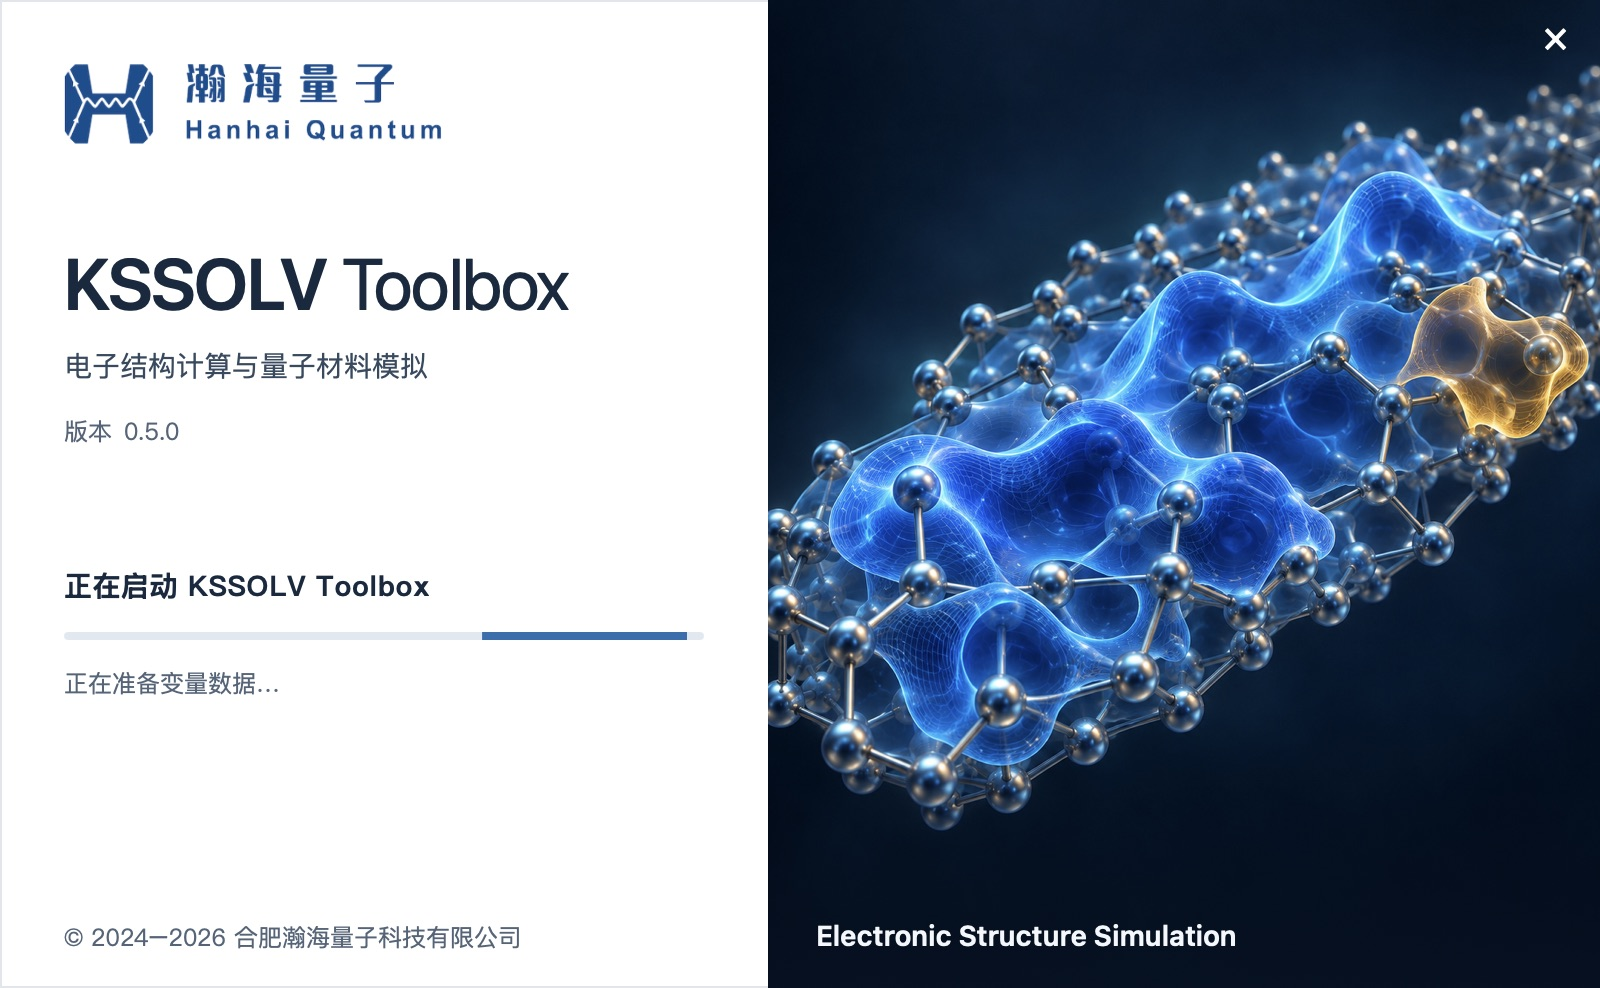
\includegraphics[width=122mm]{publication-assets/crop-6bf7d3c41caf0892911f.png}
\caption{KSSOLV Toolbox V0.5.0 獨立應用的啟動卡片，顯示產品版本與載入狀態。}
\label{fig:desktop-startup-050}
\end{figure}

啟動卡片收起後，主視窗顯示專案瀏覽器、功能區和中央文件區，可以開始下面的版本檢查與專案練習。

\subsection{確認介面和版本}

主視窗出現後，先找到上方的\ui{主頁}功能區和左側\ui{專案瀏覽器}，再選擇\ui{主頁 → 幫助 → 關於 KSSOLV}核對產品版本。本書適用版本為 V0.5.0。介面語言在\ui{主頁 → 設定 → 通用}中選擇，修改後下次啟動生效。

圖\ref{fig:install-workspace-overview}展示空專案中展開主要面板後的完整介面。上方功能區用於匯入結構、建立工作流和執行任務；左側專案瀏覽器列出工作內容，下方資訊瀏覽器顯示所選物件的屬性。中央文件區顯示歡迎文字，匯入結構後會出現三維檢視；右側配置編輯器填寫引數，模擬瀏覽器顯示執行輸出。底部命令列視窗提供互動命令入口，圖形教程不要求在這裡輸入命令。

\begin{figure}[!htb]
\centering
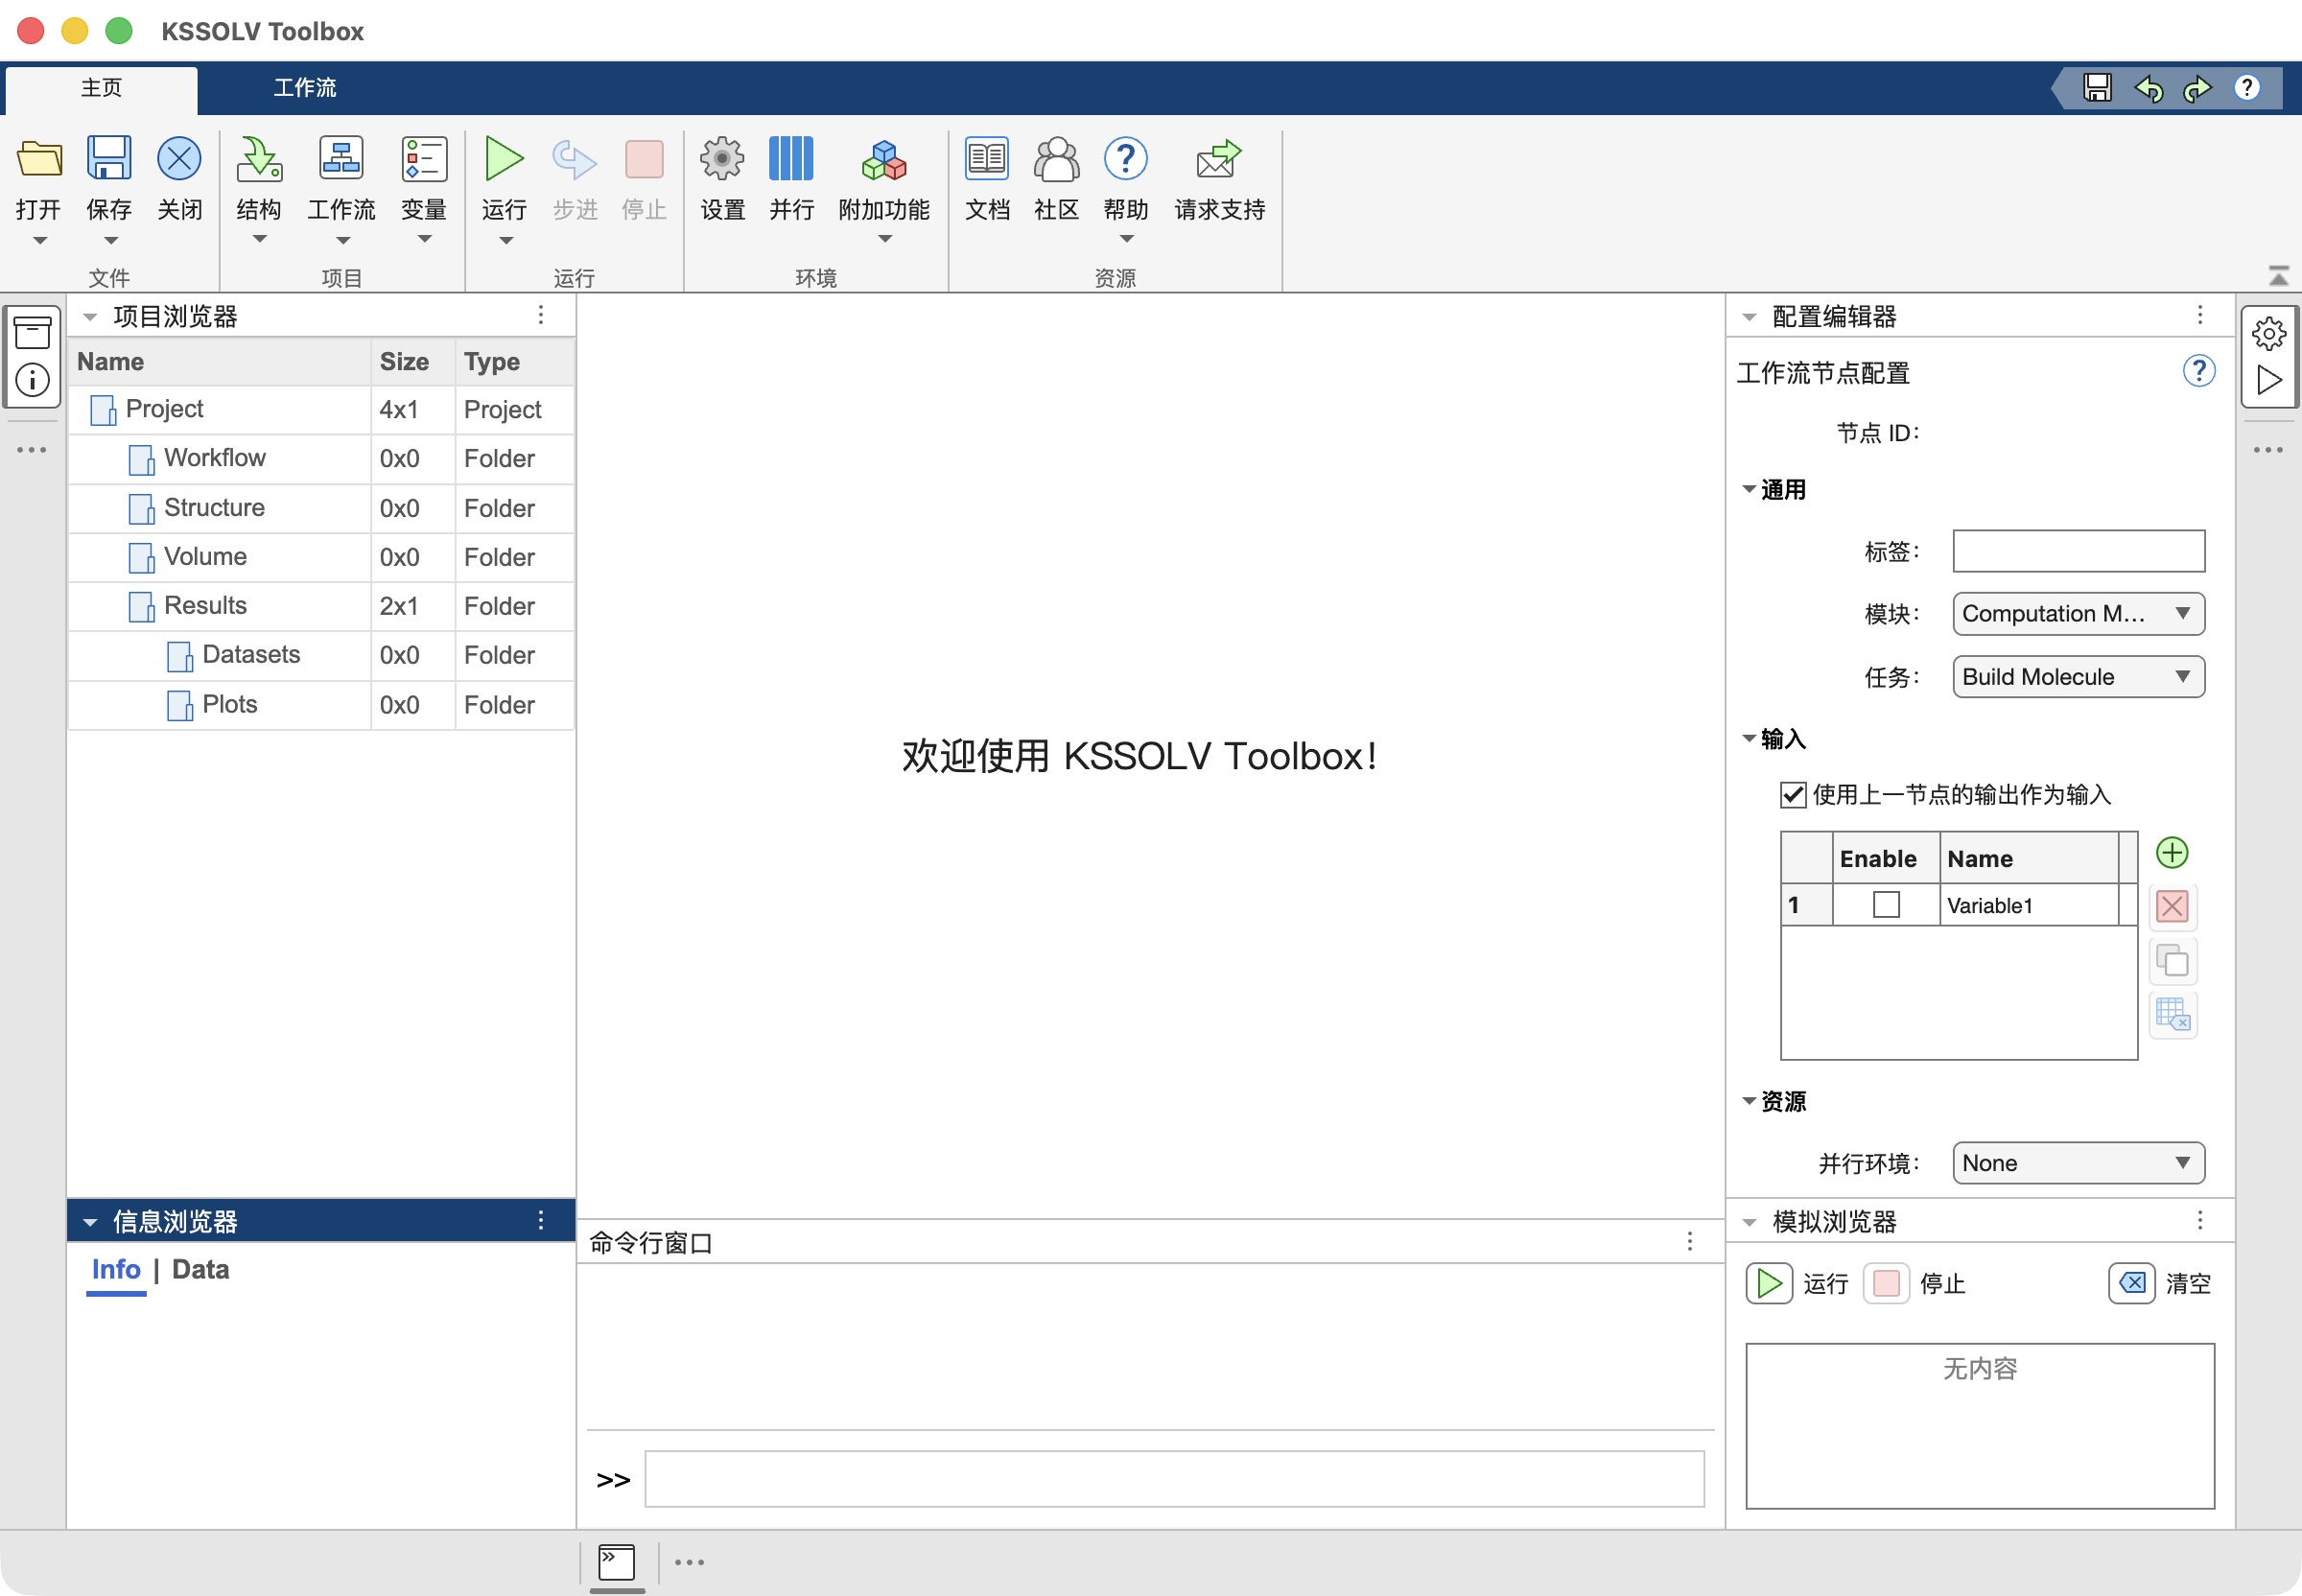
\includegraphics[width=\linewidth]{publication-assets/crop-c885d8ed3b1bcd221501.png}
\caption{獨立應用程式的完整工作區佈局。專案、資訊、配置、模擬和命令列面板均已展開；中央尚未開啟結構或工作流文件。}
\label{fig:install-workspace-overview}
\end{figure}

首次進入時，部分面板處於收起狀態。可以透過左右側邊按鈕組展開相應區域，或從省略號的\ui{開啟面板}列表選擇需要的面板。首次練習主要使用結構匯入與專案儲存入口；各區域的具體用法見第\ref{ch:workspace}章。

\subsection{建立一個可以重新開啟的專案}

這項練習只檢查檔案與介面，不需要執行計算。準備隨書的 \file{examples/silicon.cif}，也可使用自己的小型 CIF、XYZ 結構檔案。使用隨書矽結構時，可直接與第\ref{ch:workspace}章的工作區練習銜接。

\begin{steps}
\item 選擇 \ui{主頁 → 結構 → 從檔案匯入結構…}，選中準備好的結構檔案。
\item 確認結構名稱出現在專案瀏覽器中，中央三維檢視顯示原子。
\item 用滑鼠拖動旋轉檢視，再用滾輪調整大小，確認結構能夠完整顯示。
\item 點選 \ui{儲存}，在自己的工作目錄輸入 \file{first-project.ks}。
\item 確認儲存完成後關閉當前專案，再透過 \ui{開啟專案…} 開啟剛儲存的檔案。
\item 檢查專案瀏覽器和結構文件，確認此前匯入的結構仍在。
\end{steps}


完成這項練習後，即可使用結構匯入、三維顯示和專案儲存功能。第一次電子結構計算見第~\ref{ch:first}~章。

\section{遇到問題時先檢查什麼}

如果程式未能啟動，檢查安裝包是否匹配處理器架構，Runtime 是否為安裝器要求的版本。需要反饋問題時，提供 Toolbox 版本、作業系統、安裝位置和視窗中的完整提示。

如果主視窗出現但三維結構沒有顯示，先用本章的小結構重試，並觀察是否有明確的圖形提示。線上版還需使用能執行 WebGL 的瀏覽器。若檔案匯入後沒有新增專案項，核對結構檔案格式和內容。

如果儲存時找不到檔案，先確認儲存位置：獨立應用與 MATLAB\regmark{} 工具箱使用本機目錄，\ksonline{} 使用伺服器上的工作目錄。雲端“檔案”面板的操作，以及上傳與下載練習，見第\ref{ch:online}章。

\subsection{為後續練習整理檔案}

為專案建立固定目錄，分別儲存原始結構和工作專案，保留原始檔案的來源與名稱。在結構準備、引數檢查和結果整理完成時另存專案副本，便於回到已有階段。跨計算機傳遞時優先使用完整的 \file{.ks} 專案；單獨的結構檔案通常不包含工作流和計算結果。

